% !TEX encoding = UTF-8 Unicode
\chapter{Digitale Bildung}

\section{Einleitung und Motivation}

blahblah blah ich bin so motiviert

\section{Stand der Dinge}

Um ein Bild über den Stand der Dinge des Informatik-Unterrichts zu bekommen wurde hier der Bildungsplan für Baden-Württemberg untersucht. Genauer gesagt der ab 2016 gültige Bildungsplan für die Grundschule und gemeinsamen Teil der Sekundarstufe I. Mit diesen beiden Schulstufen ist der Schulweg eines jeden Schülers in Baden-Würrtemberg abgedeckt und eignet sich somit sich ein Bild über den Bildungsstand der Allgemeinhiet Im Bereich Informtaik zu machen. Denn damit sind alle Schüler von der ersten bis zu 10. Klasse abgedeckt und ist somit die Bildung die theoretisch jeder Schüler in Baden-Würtemberg bekommt. Hier wird untersucht, welche gebiete der Informatik an den öffentlichen Schulen unterrichtet wird, und wie diese unterrichted werden, um eine Aussage darüber zu treffen, ob die aus der Einleitung gennanten Punkte bereits umgesetzt wurden.

\subsection{Grundschule}
Im Bildungsplan der Grundschule gibt es keinen eigenen Abschnitt für das Fach Informatik\cite{Fachuebersicht}.Und auch in ferner verwandten Fächer wie der Mathematik\cite{Mathematik} oder gar Sachunterricht\cite{Sachunterricht}  finden sich keine Teilgebiete die unbedingt mit der Informatik zu tun haben. Daraus kann der Schluss gezogen werden, dass die Infromatik als Fach in der Grundschule vom aktuellen Bildungsplan von Baden-Würtemberg so nicht vorgesehn ist.

\subsection{Sekundarstufe I}
Ab der Sekundarstufe I (also 5. - 10. Klasse) ist im gemeinsamen Bildungsplan für alle Schulsystem ein eigenes Fach für die Informatik vorgesehn, dass in mehrere Kompetenzen aufgegliedert wurde\cite{Informatik}. Folgende Infografik wurde zu diesen Verschiedenen Kompetenzen veröffentlicht:

\begin{figure}[ht]
	\centering
	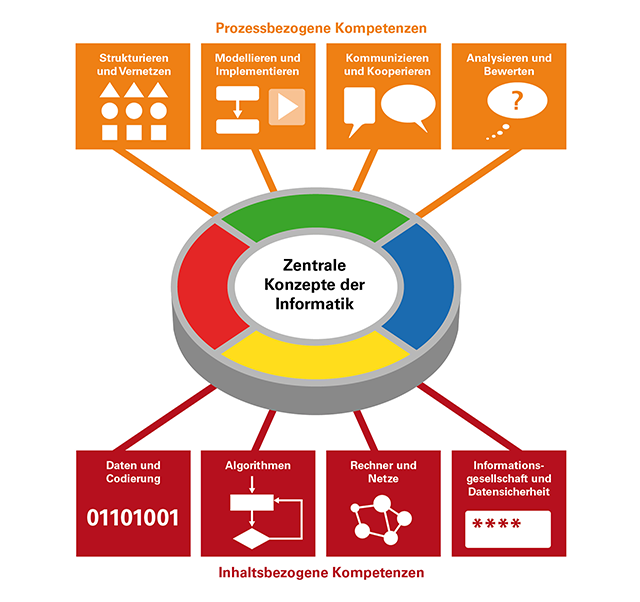
\includegraphics[width=\textwidth,height=\textheight,keepaspectratio]{images/BildungsplanInformatik.png}
	\caption{Infografik zu den Inhalten des Bildungsplans 2016 von Baden-Würtemberg für das Fach Informatik}
	\label{Bildungsplan Infromatik Infografik}
\end{figure}

Im folgenden wird auf die verschieden Kompentenzen eingegangen deren Inhalte, sowie deren Art und Weise wie diese beigebracht werden, erläutert

\subsubsection{Strukturieren und Vernetzen}
O --> []

\subsubsection{Modellieren und Implementieren}
das runde muss ins eckige

\subsubsection{Kommunizieren und Kooperieren}
hallo ich kann reden

\subsubsection{Analysieren und Bewerten}
ich finde die ganze Sache hier ja richtig behindert

\subsubsection{Daten und Codierung}
010101010

\subsubsection{Algorithemn}
Wenn du mir aufn sack gehst hau ich dir aufs maul

\subsubsection{Rechner und Netze}
der ganze deep-web shit

\subsubsection{Informationsgesellschaft und Datensicherheit}
free candy is halt nich immer free candy

\subsection{Fazit}
Nach der Erläuterung des aktuellen Bildungsplans sind einige aus der Einleitung genannten Punkte doch breits schon umgesetzt worden. Aberes ist natürlich auch nicht davon ausgehen, dass ein Fach auch genau so unterrichtet wird, wie es im Bildungsplan vorgeschrieben wird. Theorie und Praxis unterscheiden sich in der Realität öfters und es gibt noch viele andere Faktoren die sich auf den Lerninhalt eines Schüler auswriken, wie z.B. Die Kompetenz des Lehrers oder der Wille zu Lernen bei den Schülern. Ein weiterere recht auffälliger Punkt, der bei der AUfkam war, dass der vorherige Bildungsplan zum Bildungsplan 2016 aus dem Jahr 2004 stammt. Wenn dieses Tempo beibehalten wird, kann man nicht vor dem Jahr 2028 mit einem neuen Bildungsplan rechnen. Im Feld der Informatik kann man es sich aber einfach nicht Leisten 12 Jahre lang nichts zu tun, während sich in der neue Technologien entwicklen und neue Paradigmen entstehen, während die alten langsam an relevanz verlieren und schließlich verschwinden. Deshalb sollte sich ein Bildungsplan in deutlich kleineren Abständen erneuern, wenn der Ziel doch sein soll, die nächste Generation auf die Real Welt loszulassen. Ein großer Punkt aus der Einleitung der nicht vom Bildungsplan abgedeckt wird ist eine Form von Logik-Unterricht und allgemein Fächer oder EInheiten in der Grundschule die mit Informatik oder Logik zu tun haben. Deshalb wäre genau das ein Potential das man noch erarbeiten könnte.

\section{Logik-Unterricht in der Grundschule}
dat können die kleinen scheißer auch!